%!TeX encoding = UTF-8
%!TeX program = xelatex
\documentclass[notheorems, aspectratio=54]{beamer}
% aspectratio: 1610, 149, 54, 43(default), 32
\usepackage[utf8]{inputenc}
\usepackage[vietnamese]{babel}
\usepackage{latexsym}
\usepackage{amsmath,amssymb}
\usepackage{mathtools}
\usepackage{color,xcolor}
\usepackage{graphicx}
\usepackage{algorithm}
\usepackage{amsthm}
\usepackage{lmodern} % 解决 font warning
% \usepackage[UTF8]{ctex}
\usepackage{animate} % insert gif

\usepackage{lipsum} % To generate test text 
\usepackage{ulem} % 下划线,波浪线

\usepackage{listings} % display code on slides; don't forget [fragile] option after \begin{frame}

% ----------------------------------------------
% tikx
\usepackage{framed}
\usepackage{tikz}
\usepackage{pgf}
\usetikzlibrary{calc,trees,positioning,arrows,chains,shapes.geometric,%
	decorations.pathreplacing,decorations.pathmorphing,shapes,%
	matrix,shapes.symbols}
\pgfmathsetseed{1} % To have predictable results
% Define a background layer, in which the parchment shape is drawn
\pgfdeclarelayer{background}
\pgfsetlayers{background,main}

% define styles for the normal border and the torn border
\tikzset{
	normal border/.style={orange!30!black!10, decorate, 
		decoration={random steps, segment length=2.5cm, amplitude=.7mm}},
	torn border/.style={orange!30!black!5, decorate, 
		decoration={random steps, segment length=.5cm, amplitude=1.7mm}}}

% Macro to draw the shape behind the text, when it fits completly in the
% page
\def\parchmentframe#1{
	\tikz{
		\node[inner sep=2em] (A) {#1};  % Draw the text of the node
		\begin{pgfonlayer}{background}  % Draw the shape behind
			\fill[normal border] 
			(A.south east) -- (A.south west) -- 
			(A.north west) -- (A.north east) -- cycle;
\end{pgfonlayer}}}

% Macro to draw the shape, when the text will continue in next page
\def\parchmentframetop#1{
	\tikz{
		\node[inner sep=2em] (A) {#1};    % Draw the text of the node
		\begin{pgfonlayer}{background}    
			\fill[normal border]              % Draw the ``complete shape'' behind
			(A.south east) -- (A.south west) -- 
			(A.north west) -- (A.north east) -- cycle;
			\fill[torn border]                % Add the torn lower border
			($(A.south east)-(0,.2)$) -- ($(A.south west)-(0,.2)$) -- 
			($(A.south west)+(0,.2)$) -- ($(A.south east)+(0,.2)$) -- cycle;
\end{pgfonlayer}}}

% Macro to draw the shape, when the text continues from previous page
\def\parchmentframebottom#1{
	\tikz{
		\node[inner sep=2em] (A) {#1};   % Draw the text of the node
		\begin{pgfonlayer}{background}   
			\fill[normal border]             % Draw the ``complete shape'' behind
			(A.south east) -- (A.south west) -- 
			(A.north west) -- (A.north east) -- cycle;
			\fill[torn border]               % Add the torn upper border
			($(A.north east)-(0,.2)$) -- ($(A.north west)-(0,.2)$) -- 
			($(A.north west)+(0,.2)$) -- ($(A.north east)+(0,.2)$) -- cycle;
\end{pgfonlayer}}}

% Macro to draw the shape, when both the text continues from previous page
% and it will continue in next page
\def\parchmentframemiddle#1{
	\tikz{
		\node[inner sep=2em] (A) {#1};   % Draw the text of the node
		\begin{pgfonlayer}{background}   
			\fill[normal border]             % Draw the ``complete shape'' behind
			(A.south east) -- (A.south west) -- 
			(A.north west) -- (A.north east) -- cycle;
			\fill[torn border]               % Add the torn lower border
			($(A.south east)-(0,.2)$) -- ($(A.south west)-(0,.2)$) -- 
			($(A.south west)+(0,.2)$) -- ($(A.south east)+(0,.2)$) -- cycle;
			\fill[torn border]               % Add the torn upper border
			($(A.north east)-(0,.2)$) -- ($(A.north west)-(0,.2)$) -- 
			($(A.north west)+(0,.2)$) -- ($(A.north east)+(0,.2)$) -- cycle;
\end{pgfonlayer}}}

% Define the environment which puts the frame
% In this case, the environment also accepts an argument with an optional
% title (which defaults to ``Example'', which is typeset in a box overlaid
% on the top border
\newenvironment{parchment}[1][Example]{%
	\def\FrameCommand{\parchmentframe}%
	\def\FirstFrameCommand{\parchmentframetop}%
	\def\LastFrameCommand{\parchmentframebottom}%
	\def\MidFrameCommand{\parchmentframemiddle}%
	\vskip\baselineskip
	\MakeFramed {\FrameRestore}
	\noindent\tikz\node[inner sep=1ex, draw=black!20,fill=white, 
	anchor=west, overlay] at (0em, 2em) {\sffamily#1};\par}%
{\endMakeFramed}

% ----------------------------------------------

\mode<presentation>{
	\usetheme{CambridgeUS}
	% Boadilla CambridgeUS
	% default Antibes Berlin Copenhagen
	% Madrid Montpelier Ilmenau Malmoe
	% Berkeley Singapore Warsaw
	\usecolortheme{beaver}
	% beetle, beaver, orchid, whale, dolphin
	\useoutertheme{infolines}
	% infolines miniframes shadow sidebar smoothbars smoothtree split tree
	\useinnertheme{circles}
	% circles, rectanges, rounded, inmargin
}
% 设置 block 颜色
\setbeamercolor{block title}{bg=red!30,fg=white}

\newcommand{\reditem}[1]{\setbeamercolor{item}{fg=red}\item #1}

% 缩放公式大小
\newcommand*{\Scale}[2][4]{\scalebox{#1}{\ensuremath{#2}}}

% 解决 font warning
\renewcommand\textbullet{\ensuremath{\bullet}}

% ---------------------------------------------------------------------
% flow chart
\tikzset{
	>=stealth',
	punktchain/.style={
		rectangle, 
		rounded corners, 
		% fill=black!10,
		draw=white, very thick,
		text width=6em,
		minimum height=2em, 
		text centered, 
		on chain
	},
	largepunktchain/.style={
		rectangle,
		rounded corners,
		draw=white, very thick,
		text width=10em,
		minimum height=2em,
		on chain
	},
	line/.style={draw, thick, <-},
	element/.style={
		tape,
		top color=white,
		bottom color=blue!50!black!60!,
		minimum width=6em,
		draw=blue!40!black!90, very thick,
		text width=6em, 
		minimum height=2em, 
		text centered, 
		on chain
	},
	every join/.style={->, thick,shorten >=1pt},
	decoration={brace},
	tuborg/.style={decorate},
	tubnode/.style={midway, right=2pt},
	font={\fontsize{10pt}{12}\selectfont},
}
% ---------------------------------------------------------------------

% code setting
\lstset{
	language=C++,
	basicstyle=\ttfamily\footnotesize,
	keywordstyle=\color{red},
	breaklines=true,
	xleftmargin=2em,
	numbers=left,
	numberstyle=\color[RGB]{222,155,81},
	frame=leftline,
	tabsize=4,
	breakatwhitespace=false,
	showspaces=false,               
	showstringspaces=false,
	showtabs=false,
	morekeywords={Str, Num, List},
}

% ---------------------------------------------------------------------
%
\author{\textbf{Nguyễn Hoàng Đức, Lê Nhựt Nam, Nguyễn Viết Dũng}\newline\newline
	GV Lý thuyết: \textbf{PGS. TS} Lê Hoàng Thái\newline
	GV Hướng dẫn: Nguyễn Ngọc Thảo, Lê Thanh Phong}
\title{SINH TRẮC HỌC GIỌNG NÓI\newline VOICE BIOMETRICS}

%
\setbeamertemplate{caption}[numbered]
% footer
\makeatletter
\setbeamertemplate{footline}
{
	\leavevmode%
	\hbox{%
		\begin{beamercolorbox}[wd=1\paperwidth,ht=2.25ex,dp=1ex,right]{institute in head/foot}%
			\usebeamerfont{title in head/foot} 
			\insertframenumber{} / \inserttotalframenumber\hspace*{2ex} 
	\end{beamercolorbox}}%
}
\makeatother

%
\newcommand{\argmax}{\arg\!\max}

\begin{document}

\begin{frame}
	\centering
	ĐẠI HỌC QUỐC GIA THÀNH PHỐ HỒ CHÍ MINH
	
	ĐẠI HỌC KHOA HỌC TỰ NHIÊN
	
	KHOA CÔNG NGHỆ THÔNG TIN
	
	BỘ MÔN KHOA HỌC MÁY TÍNH
	\titlepage
\end{frame}
\begin{frame}{Nội dung trình bày}
	\textbf{A. Trình bày nội dung tìm hiểu được từ Chapter 8 - Voice Biometrics}
	\begin{itemize}
		\item Giới thiệu
		\item Xác định những thông tin trong tín hiệu giọng nói
		\item Rút trích đặc trưng và Phân tách dữ liệu
		\item Nhận dạng giọng nói phụ thuộc văn bản
		\item Nhận dạng giọng nói không phụ thuộc văn bản
		\item Ứng dụng
	\end{itemize}
\end{frame}
\begin{frame}{Nội dung trình bày}
	\textbf{B. Trình bày các phương pháp STATE OF THE ART của Voice Recognition}
	\begin{itemize}
		\item Động lực nghiên cứu khoa học
		\item Kho ngữ liệu/ Cơ sở dữ liệu 
		\item Phát biểu bài toán
		\item Các công trình liên quan
		\item Demo
		\item Tài liệu tham khảo
	\end{itemize}
\end{frame}

\section{Chapter 8 - Voice Biometrics}
\subsection{Giới thiệu về Sinh trắc học Giọng nói}
\begin{frame}{Giới thiệu}
	\begin{itemize}
		\item Giọng nói (Voice/Speech) là một đặc điểm sinh trắc học (nhân trắc học) dễ dàng tiếp cận nhất mà không cần phải có thêm thiết bị thu nhận và hệ thống truyền dẫn.
		\item Có lợi thế khi áp dụng vào các hệ thống điều khiển từ xa
		\item Giọng nói không chỉ liên quan đến các đặc trưng cá thể mà còn liên quan với môi trường xung quanh và vấn đề xã hội, do vậy việc sản sinh giọng nói là một kết quả của một quá trình hết sức phức tạp.
	\end{itemize}
\end{frame}
\subsection{Xác định những thông tin trong tín hiệu giọng nói}
\begin{frame}
	Những thông tin nhận dạng trong tín hiệu giọng nói
	\begin{itemize}
		\item Idiolectal characteristics: cách phát âm phản ánh khu vực bạn đang sống hoặc đã sống và các phong cách nói khác nhau thay đổi một cách tinh vi tùy thuộc vào người bạn đang nói đến.
		\item Phonotactics characteristics: Mô tả cách sử dụng của người nói của các đơn vị ngữ âm và khả năng nhận ra khả dụng. 
		\item Prosody characteristics: Prosody (ngữ điệu), là sự kết hợp của năng lượng tức thời, âm điệu, tốc độ nói và thời lượng đơn vị để cung cấp cho lời nói sự tự nhiên, đầy đủ ý nghĩa và giọng điệu cảm xúc.
		\item Short-term spectral characteristics: liên quan trực tiếp với hành động phát âm đơn lẻ, quan hệ với tạo ra ngữ âm và cũng liên quan đến sinh lý cá nhân của quá trình phát sinh giọng nói. Đây là một thông tin nhận dạng quan trọng
	\end{itemize}
\end{frame}

\subsection{Rút trích đặc trưng và phân tách dữ liệu}
\begin{frame}{Phân tích cửa sổ (Short-term Analysis)}
	Các tín hiệu giọng nói thường thay đổi liên tục nên người ta thường giới hạn cửa sổ phân tích, thường dùng cửa sổ dạng cosine như hamming hoặc hanning, với độ dài ngắn từ 20 đến 40 mili giây, thường được gọi là tín hiệu giả tĩnh trên mỗi khung.
	\begin{figure}[h!]
		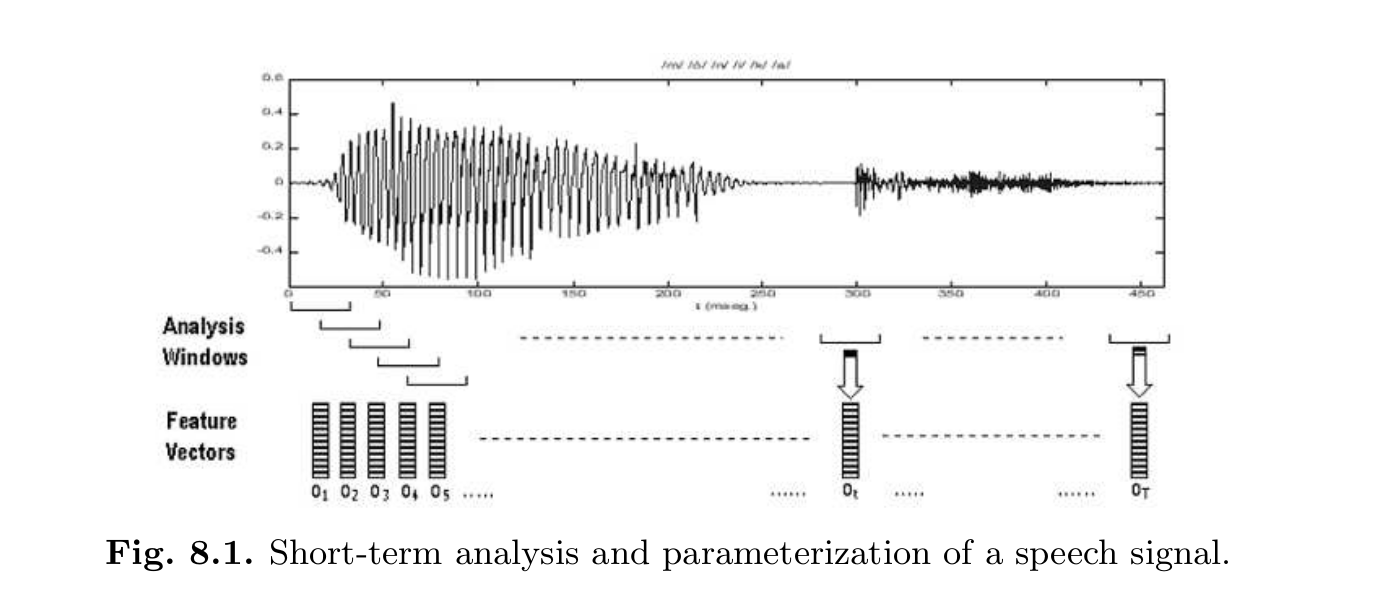
\includegraphics[width=0.9\linewidth]{images/figure_8_1.png}
		\caption{Handbook of Biometrics, page 155}
		\label{fig:writing-thesis}
	\end{figure}
\end{frame}

\begin{frame}{Tham số hóa}
	Tham số hóa bằng cách dùng Linear Predictive Coding (LPC): là một phương pháp được sử dụng hầu hết trong xử lý tín hiệu âm thanh và xử lý giọng nói để biểu diễn đường bao phổ của tín hiệu số của tiếng nói ở dạng nén, sử dụng thông tin của mô hình dự đoán tuyến tính.
	\begin{figure}[h!]
		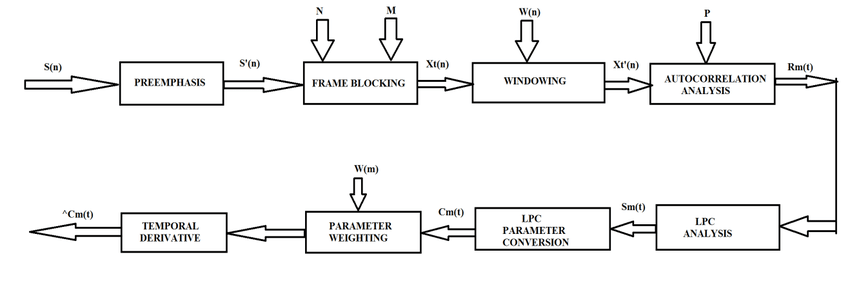
\includegraphics[width=0.9\linewidth]{images/Block-diagram-of-LPC-Linear-Predictive-Coding.png}
		\caption{Handbook of Biometrics, page 162}
		\label{fig:writing-thesis}
	\end{figure}
\end{frame}
\begin{frame}{Tham số hóa}
	Tham số hóa bằng cách dùng Mel-Frequency based Cepstral Coefficients (MFCC): MFCC là một kỹ thuật rút trích đặc trưng giọng nói được dùng nhiều trong các mô hình nhận dạng giọng nói, nó cho ra các kết quả là các hệ số (Coefficients) của cepstral từ Mel Filter trên phổ từ dữ liệu âm thanh giọng nói.
	 $$\text{speech signal} \Rightarrow \text{spectrum} \Rightarrow \text{mel-freq filter} \Rightarrow \text{cepstral}$$
	\begin{figure}[H]
		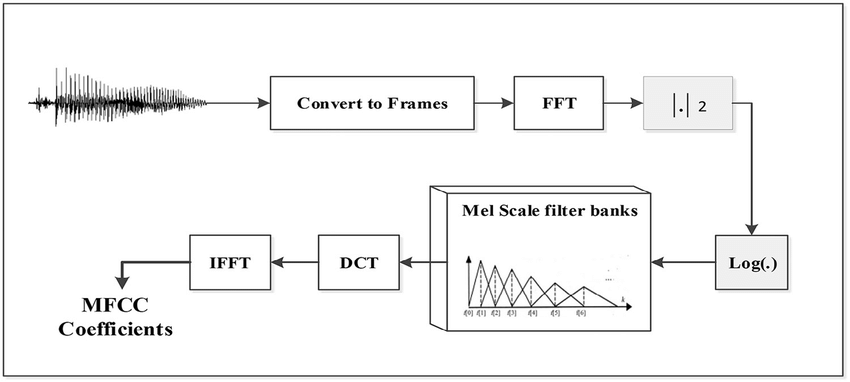
\includegraphics[width=0.75\linewidth]{images/Extraction-Mel-frequency-cepstral-coefficients-MFCC-from-the-audio-recording-signals.png}
		\label{fig:writing-thesis}
	\end{figure}
\end{frame}
\begin{frame}{Phân tích ngữ âm và tách từ}
	Mô hình Hidden Markov (HMM - Hidden Markov Models) là công cụ thành công nhất và được sử dụng rộng rãi (ngoại trừ một số kiến trúc ANN) để mã hóa ngữ âm, âm tiết và từ, nghĩa là dịch từ lời nói được lấy mẫu thành một căn chỉnh thời gian dãy các đơn vị ngôn ngữ.
	\begin{figure}[h!]
		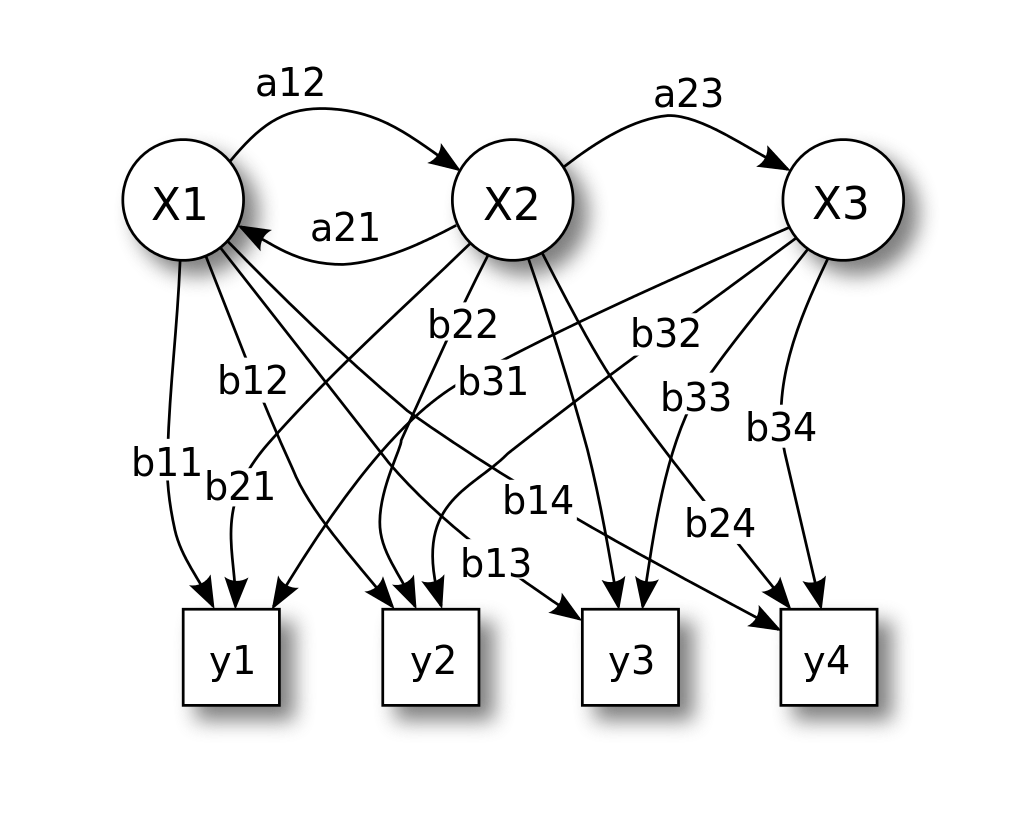
\includegraphics[width=0.6\linewidth]{images/1024px-HiddenMarkovModel.svg.png}
		\caption{Sơ đồ mô hình Markov ẩn}
		\label{fig:writing-thesis}
	\end{figure}
	
\end{frame}
\begin{frame}{Phân tách ngữ điệu}
	Dựa trên cơ sở là cao độ và năng lượng ở từng frame
	\begin{itemize}
		\item Cao độ: xác định bằng phương pháp tự động tương quan, phân rã cepstral dựa trên một số phương thức làm mịn bằng bộ lọc.
		\item Năng lượng: Năng lượng cửa sổ thu được rất dễ dàng thông qua định lý Parseval.
	\end{itemize}
\end{frame}

\subsection{Nhận dạng giọng nói phụ thuộc văn bản}
\begin{frame}{Giới thiệu}
	Công nghệ nhận dạng giọng nói phụ thuộc văn bản, sử dụng nội dung từ vựng của giọng nói phát
	ra để nhận dạng giọng nói, ứng dụng chính của hệ thống này trong các hệ thống tương tác, nơi cần có sự hợp tác từ người dùng để xác thực danh tính của họ.
	
	Phân loại
	\begin{itemize}
		\item Hệ thống văn bản tĩnh: nội dung từ vựng trong ghi danh và các mẫu nhận dạng luôn giống
		nhau.
		\item Hệ thống văn bản động: tạo ra một lời nhắc mật khẩu được tạo ngẫu nhiên khác nhau mỗi
		khi người dùng được xác minh (hệ thống nhắc bằng văn bản)
	\end{itemize}
\end{frame}
\begin{frame}{Phương pháp thực hiện}
	Có hai phương pháp thường được dùng:
	\begin{itemize}
		\item Phương pháp dựa trên khuôn mẫu: bao gồm một số chuỗi vector tương ứng với lời nói đăng
		ký và việc nhận dạng được thực hiện bằng cách so sánh lời nói xác minh với lời nói đăng ký.
		\item Phương pháp thống kê: Nổi bật nhất là mô hình Markov ẩn (HMM), cho phép chọn đơn vị tiếng nói từ đơn vị âm vị phụ đến từ và cho phép thiết kế hệ thống nhắc văn bản.
	\end{itemize}
\end{frame}

\subsection{Nhận dạng giọng nói không phụ thuộc văn bản}
\begin{frame}{Giới thiệu}
	\qquad Công nghệ nhận dạng giọng nói độc lập với văn bản cố gắng giảm thiểu ảnh hưởng của nội dung từ vựng vốn được coi là không xác định đối với khả năng nhận dạng của giọng nói, điều này trái ngược với hệ thống nhận dạng giọng nói phụ thuộc văn bản, đương nhiên việc nghiên cứu và phát triển nó sẽ khó khăn hơn.
	\begin{itemize}
		\item Hệ thống cửa sổ phổ âm
		\item Hệ thống Idiolectal
		\item Hệ thống ngữ âm
		\item Hệ thống ngữ điệu
	\end{itemize}
\end{frame}
\begin{frame}{Hệ thống cửa sổ phổ âm}
	Dùng trong việc phân tích phổ trong khoảng thời gian ngắn được sử dụng để mô hình các đặc trưng người nói, nhằm mô hình hóa các “âm thanh” khác nhau mà một người có thế tạo ra
	\begin{itemize}
		\item Kỹ thuật Lượng tử hóa Vector (Vector Quantization techniques)
		\item Gaussian Mixture Model - Universal Background Model
		\item Discriminative techniques - Kỹ thuật phân tách: Artificial Neural Networks, SVM - Support Vector Machine
		\item SuperVectors, một kỹ thuật hỗn hợp GMM-SVM
	\end{itemize}
\end{frame}
\begin{frame}{Hệ thống Idiolectal}
	\begin{itemize}
		\item Doddington đã lập ra mô hình cách sử dụng từ của từng người nói cụ thể bằng cách sử dụng \textbf{n-gram} mô hình hóa các chuỗi từ và xác suất của chúng và chứng minh rằng việc sử dụng các mô hình đó có thể cải thiện hiệu suất của hệ thống GMM âm thanh/ phổ cơ bản. 
		\item Quan trọng hơn kết quả cụ thể này là thực tế là công trình này đã thúc đẩy nghiên cứu trong việc sử dụng các cấp độ thông tin cao hơn (idiolectal, phonotactic, prosodic, v.v.) để \textbf{nhận dạng giọng nói độc lập với văn bản}. 
	\end{itemize}
\end{frame}
\begin{frame}{Hệ thống ngữ âm}
	\begin{columns}
		\begin{column}{0.5\textwidth}
			Mô hình hệ thống ngữ âm
			\begin{figure}[H]
				\centering
				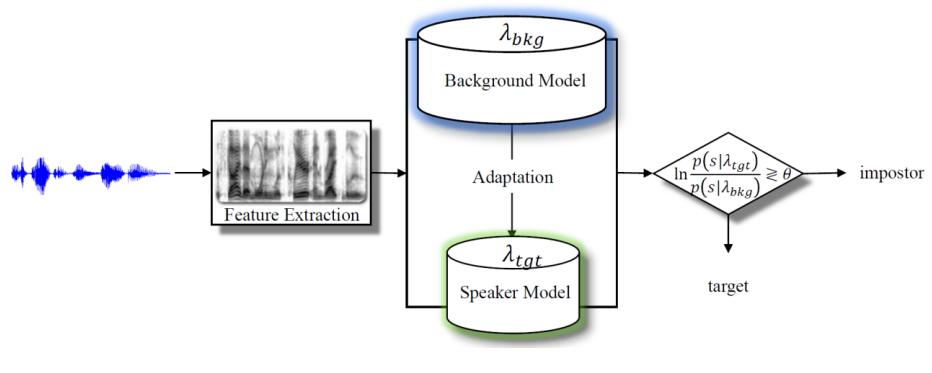
\includegraphics[width=1\linewidth]{images/diagram.png}
				\caption{Quy trình của hệ thống ngữ âm}
				\label{fig:writing-thesis}
			\end{figure}
		\end{column}
		\begin{column}{0.5\textwidth}
			\begin{itemize}
				\item Bước 1: Đầu vào là giọng nói cần xác minh
				\item Bước 2 - Token segmentation: Tách thành các đoạn t3, t4, t5, t3
				\item Bước 3: Mô hình hóa ngôn ngữ thống kê n-gram
				\begin{itemize}
					\item Huấn luyện mô hình Universal Background Phone (UBPM) $L_{U} = P(X|UBPM)$
					\item Huấn luyện mô hình Speaker Phone Models ($SPM_{i}$): $L_{S_{i}} = P(X | SPM_{i})$
				\end{itemize}
				\item Bước 4: Tính recognition score: $Score_{i} = \frac{1}{m}log\left(\frac{P(X | SPM_{i})}{P(X|UBPM)}\right)$
			\end{itemize}
		\end{column}
	\end{columns}
\end{frame}	
\begin{frame}{Hệ thống ngữ điệu}
	Mô hình hệ thống ngữ điệu
	\begin{itemize}
		\item Giai đoạn một, đối với mỗi đoạn giọng nói của đoạn thoại, quỹ đạo thời gian của các đặc điểm ngữ điệu (tần số cơ bản - hoặc cao độ- và năng lượng) được rút trích.
		\item Giai đoạn hai, cả hai đường bao đều được phân đoạn và dán nhãn bằng định lượng trung bình
		độ dốc.
	\end{itemize}
	\begin{figure}
		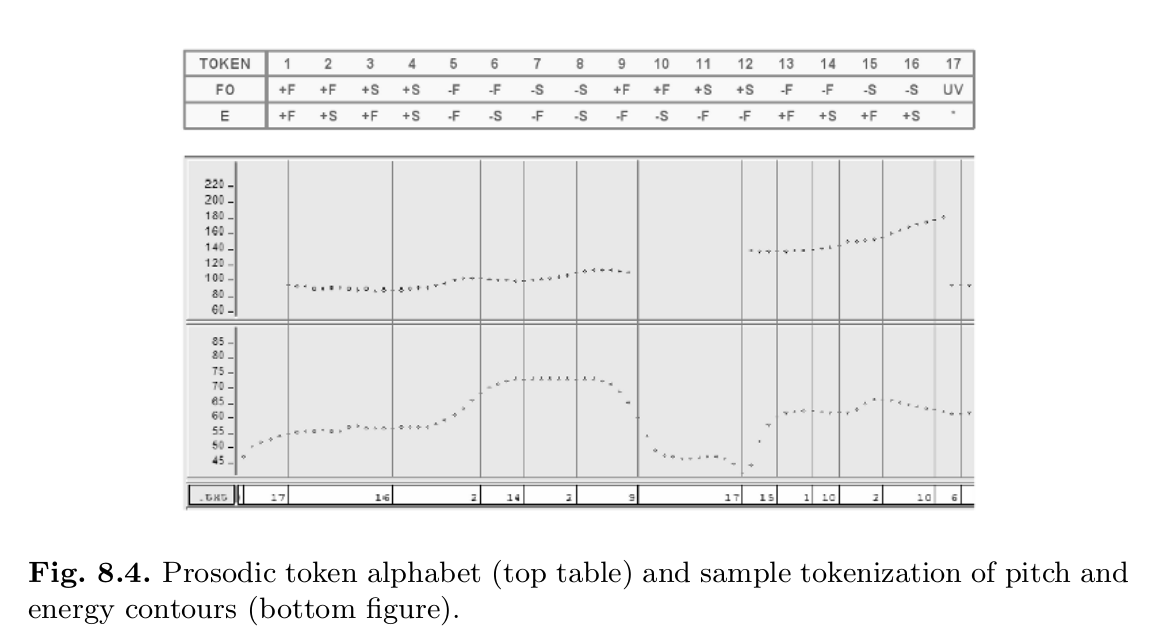
\includegraphics[width=0.75\linewidth]{images/figure_8_4.png}
		\caption{Handbook of Biometrics, page 163}
		\label{fig:writing-thesis}
	\end{figure}
\end{frame}	

\subsection{Ứng dụng của nhận dạng giọng nói}
\begin{frame}{Voice authentication}
	\begin{figure}[h!]
		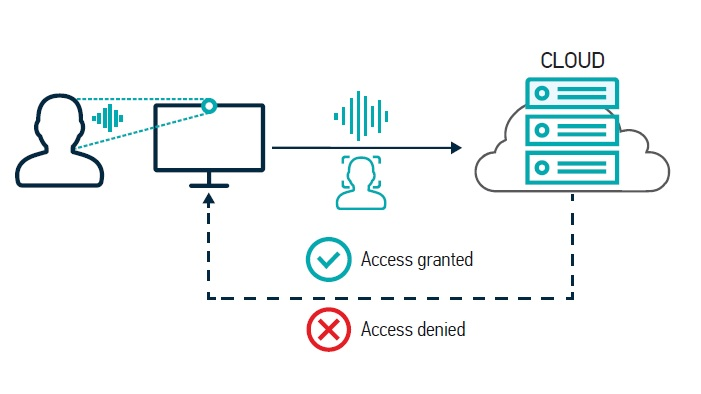
\includegraphics[width=0.9\linewidth]{images/voice_authentication.jpg}
		\caption{Ví dụ Voice authentication/ Verification}
		\label{fig:writing-thesis}
	\end{figure}
\end{frame}	
\begin{frame}{Speaker Identification and Verification}
	\begin{figure}[H]
		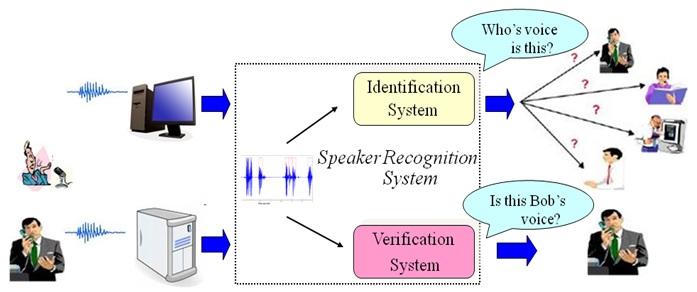
\includegraphics[width=0.9\linewidth]{images/speaker_identification_verification.jpeg}
		\caption{Ví dụ Speaker Recognition Systems}
		\label{fig:writing-thesis}
	\end{figure}
\end{frame}
\begin{frame}{Forensic speaker recognition}
	\begin{figure}[H]
		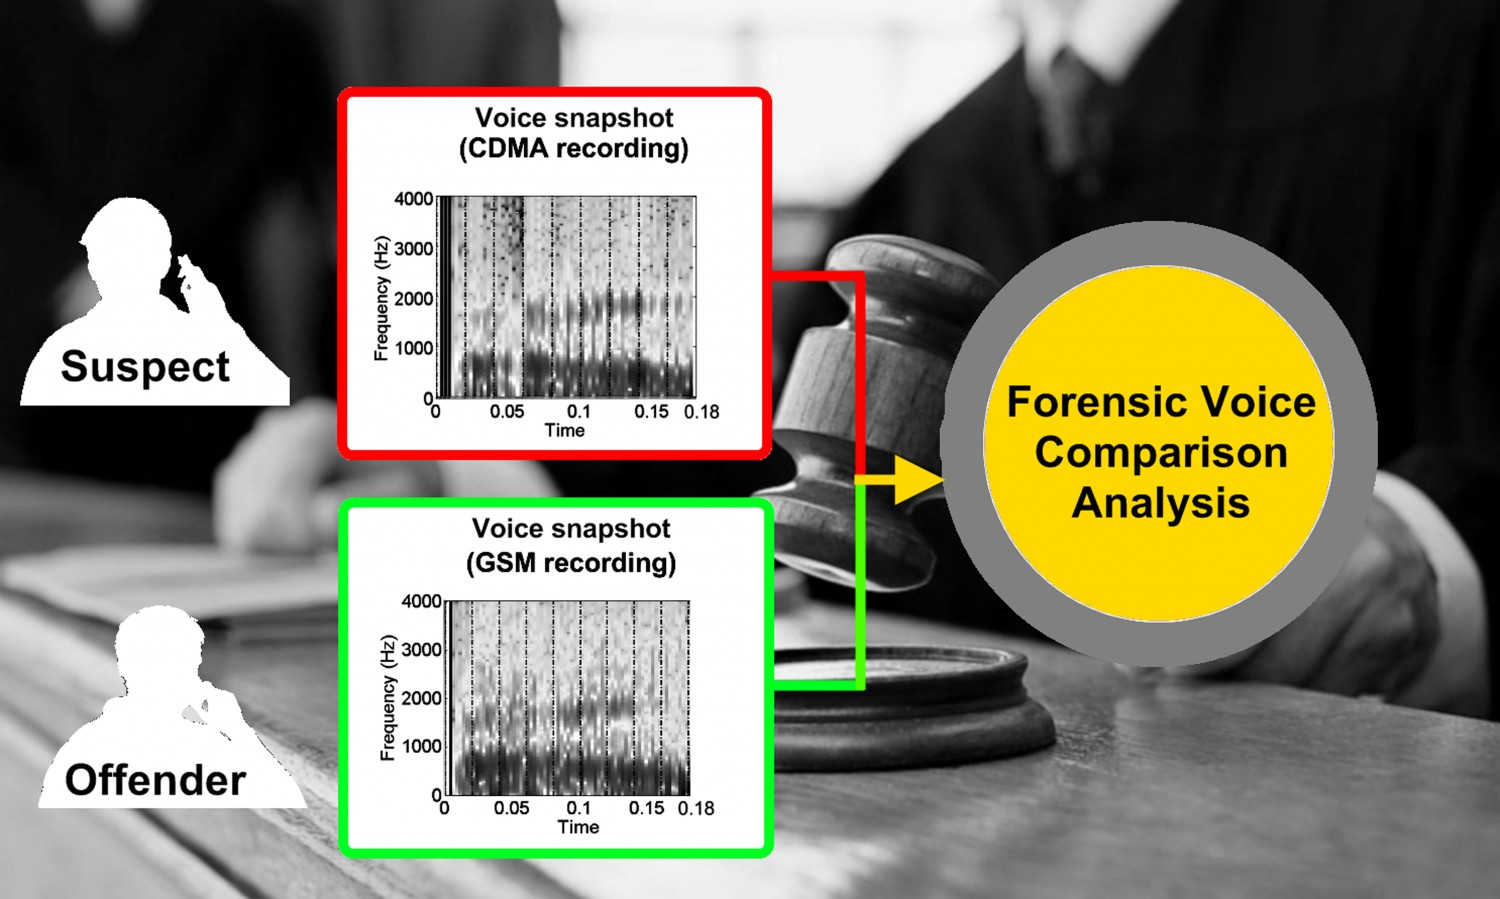
\includegraphics[width=0.9\linewidth]{images/forensic_voice.jpg}
		\caption{Ví dụ Speaker Recognition Systems}
		\label{fig:writing-thesis}
\end{figure}
\end{frame}

\section{Các phương pháp SOTA - Voice Biometrics}
\subsection{Động lực nghiên cứu khoa học}
\begin{frame}{Động lực nghiên cứu khoa học}
		\begin{itemize}
		\item Những phương pháp đã tìm hiểu từ sách Handbook of Biometrics: Voice Biometrics đã cho chúng ta cái nhìn tổng quan về lĩnh vực Nhận dạng giọng nói và những phương pháp truyền thống (tạm gọi là thời kỳ trước Deep Learning) cùng với những thông tin các công trình nghiên cứu nổi bật.
		\item Các phương pháp SOTA dựa trên việc biểu diễn i-vectors của những
		đoạn giọng nói, cải thiện đáng kể so với mô hình Gaussian Mixture
		Model-Universal Background Models
		\item Sự phát triển của Deep Learning
	\end{itemize}
\end{frame}
\subsection{Kho ngữ liệu}
\begin{frame}{Một số kho ngữ liệu lớn, nổi bật gần đây}
	\textbf{Kho ngữ liệu VCTK (Veaux et al., 2017)}
	\begin{itemize}
		\item Tên đầy đủ: SUPERSEDED - CSTR VCTK Corpus: English Multi-speaker Corpus for CSTR Voice Cloning Toolkit
		\item Tác giả/ Nhóm tác giả: Veaux Christophe, Yamagishi Junichi, MacDonald Kirsten
		\item Nhà xuất bản: University of Edinburgh. The Centre for Speech Technology Research (CSTR)
		\item Mô tả sơ lược: Tất cả dữ liệu giọng nói được ghi lại bằng cách sử dụng thiết lập ghi âm giống hệt nhau: micrô đa hướng (DPA 4035) và micrô tụ màng nhỏ với băng thông rất rộng (Sennheiser MKH 800), tần số lấy mẫu 96kHz ở 24 bit và trong một buồng phản xạ hemi của Đại học Edinburgh
	\end{itemize}
\end{frame}
\begin{frame}{Một số kho ngữ liệu lớn, nổi bật gần đây}
	\textbf{Kho ngữ liệu VoxCeleb (Nagrani et. al, 2017)}, \textbf{VoxCeleb2 (Chung et. al, 2018)}
	\begin{itemize}
		\item Tên đầy đủ: VoxCeleb2: Deep Speaker Recognition  
		\item Tác giả/ Nhóm tác giả: J. S. Chung*, A. Nagrani*, A. Zisserman
		\item Hội nghị: INTERSPEECH, 2018.  
		\item Mô tả sơ lược: Là kho ngữ liệu giọng nói lớn nhất hiện tại, VoxCeleb2 chứa hơn 1 triệu câu nói cho 6.112 người nổi tiếng, được trích xuất từ các video tải lên YouTube. Tập hợp phát triển của VoxCeleb2 không có sự trùng lặp với các đặc điểm nhận dạng trong tập dữ liệu VoxCeleb1 hoặc SITW.
	\end{itemize}
\end{frame}
\subsection{Phát biểu bài toán}
\begin{frame}{Phát biểu bài toán}
	\textbf{Tác vụ:} Định danh người nói (Speaker Identification)
	\begin{itemize}
		\item Đầu vào (Input): Dữ liệu âm thanh giọng nói (Sound)
		\item Đầu ra (Output): Danh tính của người nói (Personal Information, Label)
	\end{itemize}
	\textbf{Tác vụ:} Xác nhận người nói (Speaker Verification)
	\begin{itemize}
		\item Đầu vào (Input): Dữ liệu âm thanh giọng nói (Sound)
		\item Đầu ra (Output): Đồng ý/ Từ chối (Accept/ Deny)
	\end{itemize}
\end{frame}
\subsection{Các công trình liên quan}
\begin{frame}{Công trình tiêu biểu sử dụng d-vectors}
	Được giới thiệu trong bài báo "Deep neural networks for small footprint text-dependent speaker verification" \textbf{d-vectors} trở thành tiền đề cho hàng loạt các thành công sau này của lĩnh vực Nhận dạng giọng nói sử dụng Deep Learning.
	\textbf{Giới thiệu chung về bài báo:}
	\begin{itemize}
		\item Bài báo: Deep neural networks for small footprint text-dependent speaker verification (Một bước nhỏ trong dùng mạng học sâu cho tác vụ xác minh người nói)
		\item Nhóm tác giả: Ehsan Variani (Johns Hopkins Univ., Baltimore, MD, USA), Xin Lei, Erik McDermott, Ignacio Lopez Moreno, Javier Gonzalez-Dominguez (Google Inc., USA)
		\item Được publish tại hội nghị 2014 IEEE International Conference on Acoustics, Speech and Signal Processing (ICASSP), diễn ra tại Florence, Italy, vào năm 2014
	\end{itemize}
\end{frame}
\begin{frame}{Công trình tiêu biểu sử dụng d-vectors}
	\textbf{Mô hình d-vectors}
	\begin{figure}[H]
		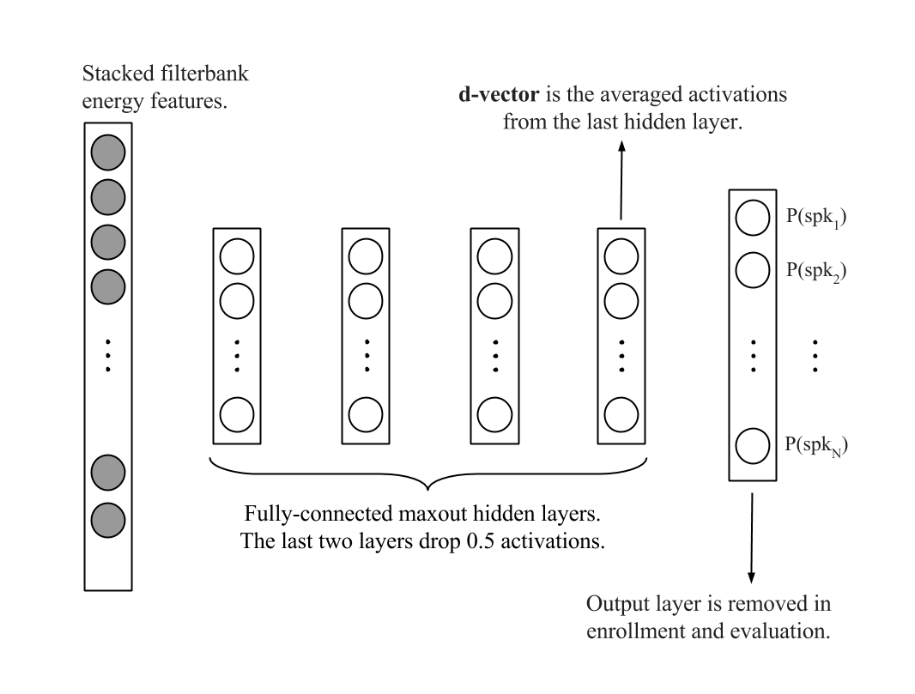
\includegraphics[width=0.7\linewidth]{images/d-vectors.png}
		\caption{Mô hình DNN với d-vectors}
		\label{fig:writing-thesis}
	\end{figure}
\end{frame}
\begin{frame}{Công trình tiêu biểu sử dụng d-vectors}
	\textbf{Phương pháp tiếp cận}
	\begin{itemize}
		\item Sử dụng Deep Neural Networks trong tác vụ xác minh người nói (Speaker Verification) để rút trích đặc trưng giọng nói và kích hoạt đặc trưng nằm lớp ẩn cuối cùng của mạng học - gọi là d-vectors (Deep Vectors)
		\item Trong giai đoạn đăng ký (Speaker Enrollment), mô hình DNN được huấn luyện sẵn được sử dụng để rút trích đặc trưng giọng nói của người nói ở lớp cuối cùng. Sau đó tính toán giá trị trung bình của những đặc trưng này, để cho ra d-vector của người nói
		\item 	Trong giai đoạn đánh giá (Evaluation Stage), một giọng nói cần được xác minh khi vào mô hình sẽ được tính toán để cho ra một d-vector. Sau đó, dùng d-vector này so sánh với những d-vector trong quá trình đăng ký để đưa ra quyết định giọng nói của người nói này có phải là đúng với danh tính đưa ra không.
	\end{itemize}
\end{frame}
\begin{frame}{Công trình tiêu biểu sử dụng d-vectors}
	\textbf{Kết quả đạt được}
	\begin{figure}[H]
		\centering
		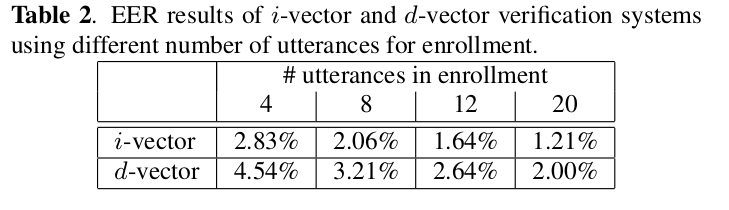
\includegraphics[width=0.75\linewidth]{images/d-vectors-result-table-02.png}
		\caption{- Deep Neural Networks for small foot-print text-dependent speaker verification - 2014}
		\label{fig:writing-thesis}
	\end{figure}
	\textbf{Nhận xét:}
	\begin{itemize}
		\item Cơ sở phương pháp, độ đo đánh giá đơn giản
		\item EER vẫn chưa tốt so với hệ thống i-vectors
	\end{itemize}
\end{frame}

\begin{frame}{Công trình tiêu biểu sử dụng j-vectors}
	\textbf{Giới thiệu chung về bài báo:}
	\begin{itemize}
		\item Bài báo: Multi-Task Learning for Text-Dependent Speaker Verification
		\item Nhóm tác giả: Nanxin Chen, Yanmin Qian, Kai Yu (Shanghai Jiao Tong University, China)
		\item Được publish tại hội nghị INTERSPEECH 2015 16th Annual Conference of the International Speech Communication Association, diễn ra tại Dresden, Germany, từ ngày 6-10 tháng 9 năm 2015
	\end{itemize}
\end{frame}
\begin{frame}{Công trình tiêu biểu sử dụng j-vectors}
	\textbf{Mô hình j-vectors}
	\begin{figure}[H]
		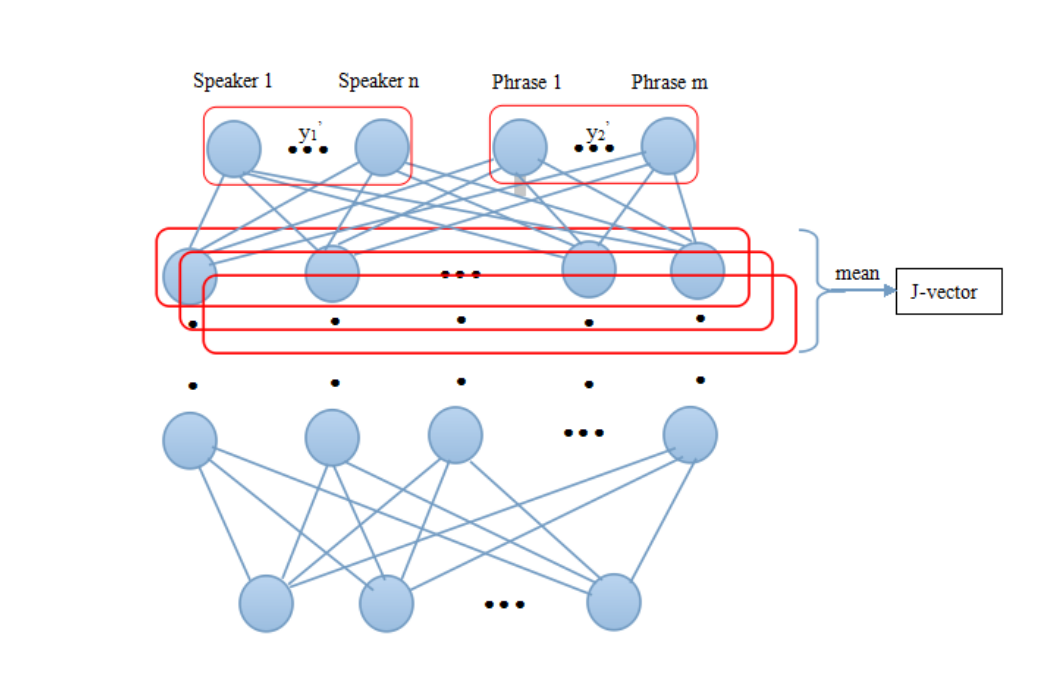
\includegraphics[width=0.7\linewidth]{images/j-vectors.png}
		\caption{Mô hình DNN với j-vectors}
		\label{fig:writing-thesis}
	\end{figure}
\end{frame}
\begin{frame}{Công trình tiêu biểu sử dụng j-vectors}
	\textbf{Phương pháp thực hiện}: Mô hình Học đa nhiệm Deep Neural Network sử dụng cho Xác minh người nói phụ thuộc văn bản được lấy ý tưởng từ việc sử dụng DNN với số lượng tham số cực lớn, một mô hình DNN có thể học cùng lúc việc phân tách văn bản, lẫn giọng nói
	
	Hai hàm mất mát ban đầu là $C_1(y_1, y_1^{'}), C_2(y_2, y_2^{'})$ được dùng để tạo thành hàm tổng mất mát:
	$$C([y_1, y_2], [y_1^{'}, y_2^{'}]) = C_1(y_1, y_1^{'}) + C_2(y_2, y_2^{'})$$
	Trong đó:
	\begin{itemize}
		\item $C_1, C_2$ lần lượt là hai cross-entropy criteria cho giọng nói và văn bản
		\item $y_1, y_2$ đại diện cho nhãn đúng của từng người nói và văn bản
		\item $y_1^{'}, y_2^{'}$ đại diện cho nhãn đầu ra (nhãn dự đoán được) của $y_1, y_2$ tương ứng
	\end{itemize}
\end{frame}
\begin{frame}{Công trình tiêu biểu sử dụng j-vectors}
	\textbf{Các kết quả đạt được}
	\begin{columns}
		\begin{column}{0.5\textwidth}
			\begin{figure}[H]
				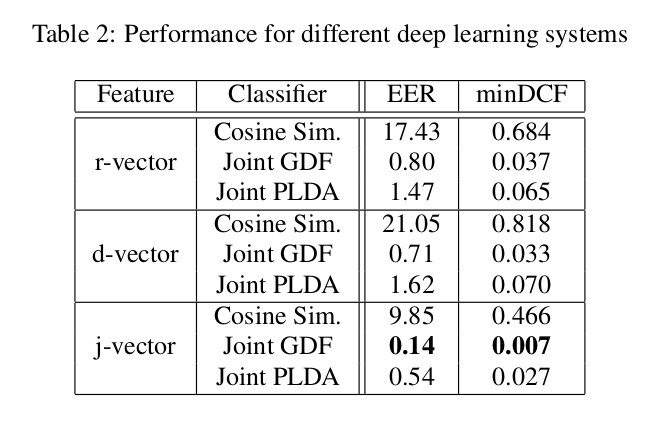
\includegraphics[width=1\linewidth]{images/j-vectors-result-table-02.png}
			\end{figure}
		\end{column}
		\begin{column}{0.5\textwidth}
			\begin{figure}[H]
				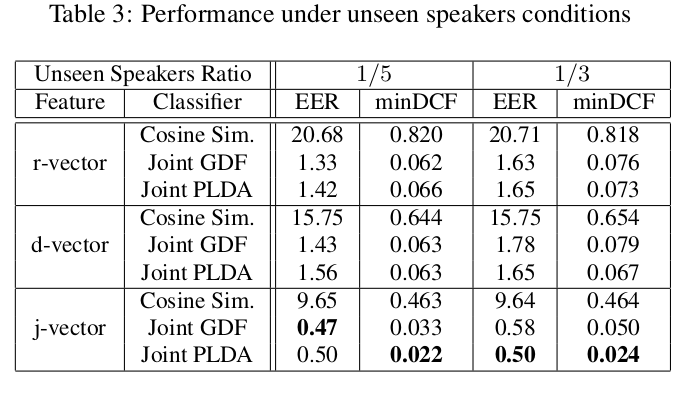
\includegraphics[width=1\linewidth]{images/j-vectors-result-table-03.png}
		\end{figure}
		\end{column}
	\end{columns}
	\textbf{Nhận xét:}
	\begin{itemize}
		\item Áp dụng học đa nhiệm (giọng nói và văn bản), rút trích ra j-vectors
		\item Kết quả tốt hơn, cho độ lỗi thấp hơn rất nhiều so với d-vector, r-vector trên tác vụ xác minh người nói phụ thuộc văn bản
	\end{itemize}
\end{frame}
\begin{frame}{Công trình tiêu biểu sử dụng x-vectors}
\textbf{Giới thiệu chung về bài báo:}
\begin{itemize}
	\item Bài báo: X-Vectors: Robust DNN Embeddings for Speaker Recognition
	\item Nhóm tác giả: 
	\begin{itemize}
		\item David Snyder, Daniel Garcia-Romero, Gregory Sell, Daniel Povey, Sanjeev Khudanpur - Center for Language and Speech Processing \& Human Language Technology Center of Excellence, The Johns Hopkins University, Baltimore, MD, USA
	\end{itemize}
	\item Được xuất bản tại hội nghị 2018 IEEE International Conference on Acoustics, Speech and Signal Processing (ICASSP), diễn ra tại Calgary, AB, Canada, năm 2018
\end{itemize}
\end{frame}
\begin{frame}{Công trình tiêu biểu sử dụng x-vectors}
	\textbf{Mô hình} x-vectors
	\begin{figure}[H]
		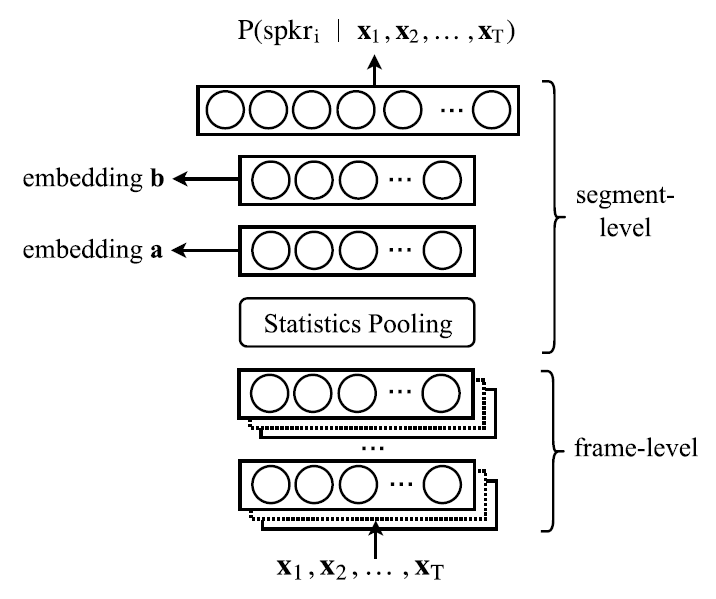
\includegraphics[width=0.65\linewidth]{images/x-vector.jpg}
		\caption{Mô hình DNN với x-vectors}
		\label{fig:writing-thesis}
	\end{figure}
\end{frame}
\begin{frame}{Công trình tiêu biểu sử dụng x-vectors}
	\textbf{Phương pháp thực hiện}
	\begin{figure}[H]
		\centering
		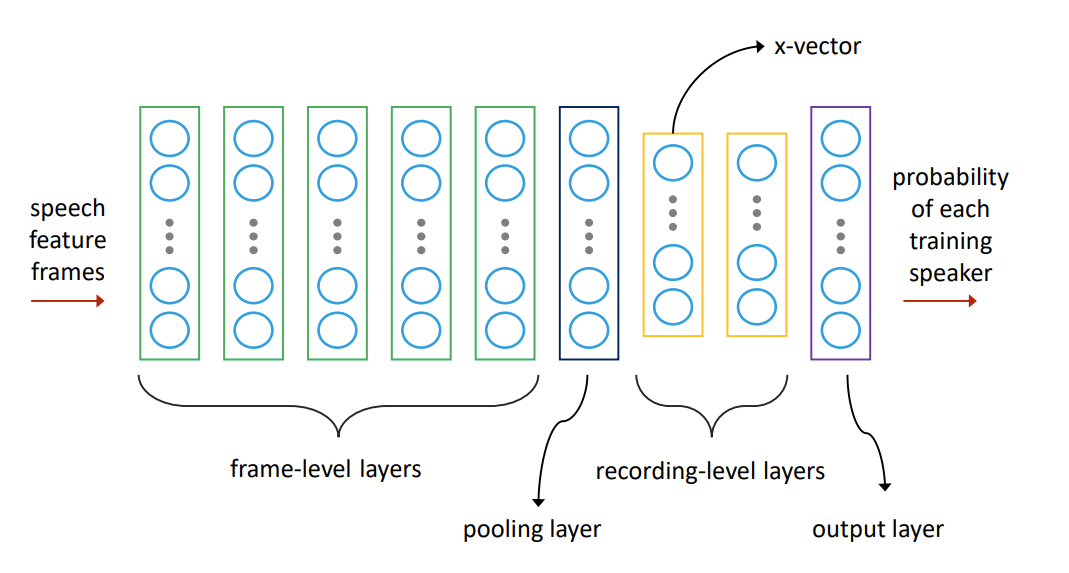
\includegraphics[width=0.75\linewidth]{images/x_vectors_dnn.png}
		\caption{From i-vectors to x-vectors – a generational change in speaker recognition illustrated on the NFI-FRIDA database - OxfordWave Research}
		\label{fig:writing-thesis}
	\end{figure}
	x-vectors sẽ được rút trích tại lớp phân đoạn 6 (segment6), ngay sau khi qua lớp tổng hợp thống kê
\end{frame}
\begin{frame}{Công trình tiêu biểu sử dụng x-vectors}
	\textbf{Các kết quả đạt được}
	\begin{figure}[H]
		\centering
		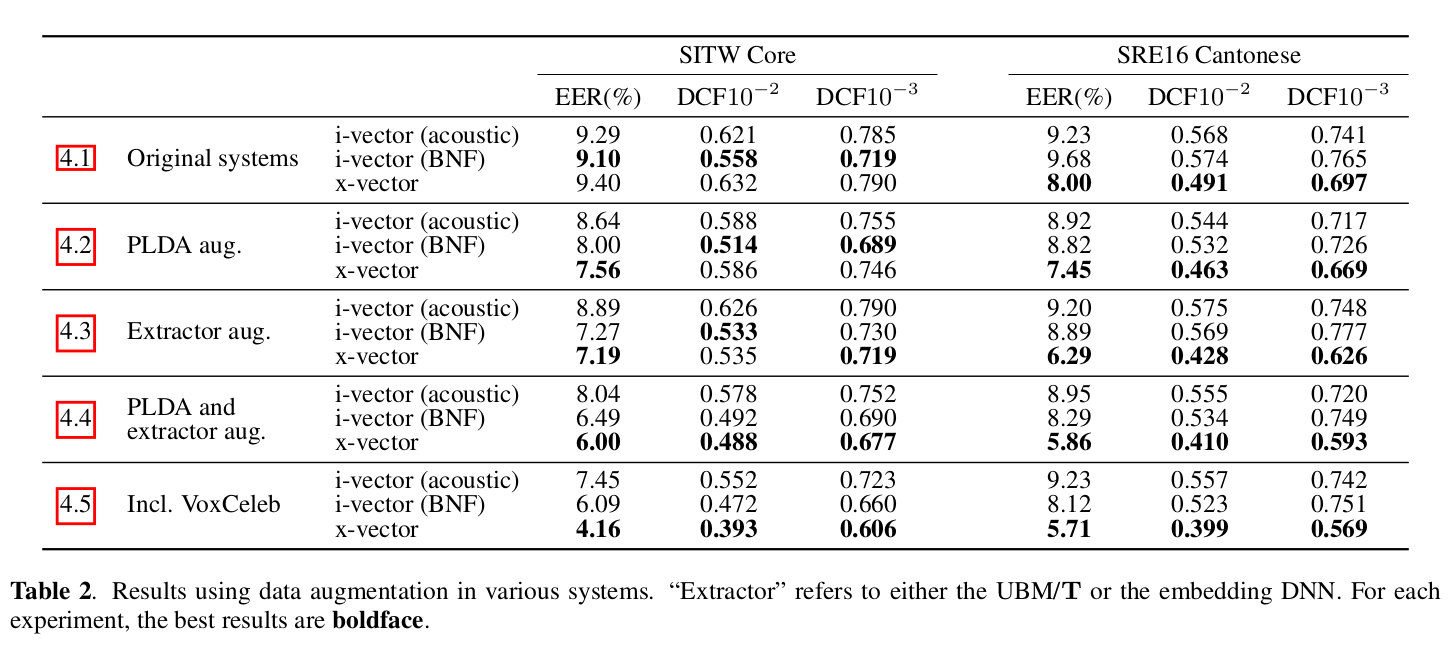
\includegraphics[width=0.75\linewidth]{images/x-vectors-result-table-02.png}
		\caption{x-vector DNN embedding architecture in (Snyder et al., 2018)}
		\label{fig:writing-thesis}
	\end{figure}
	\textbf{Nhận xét}
	\begin{itemize}
		\item Hiệu suất của x-vectors đã được chứng minh là tốt hơn đáng kể so với i-vectors, đặc biệt là ở khoảng thời gian ngắn.
	\end{itemize}
\end{frame}
\begin{frame}{So sánh d-vectors, j-vectors và x-vectors}
	\begin{table}[H]
		\centering
		\begin{tabular}{ |p{1cm} |p{3cm} | p{3cm} | p{3cm}  |}\hline
			& d-vectors & j-vectors & x-vector \\\hline
			Kỹ thuật rút trích & DNN & DNN & DNN\\ \hline
			Ví trí rút trích & Tại lớp ẩn cuối cùng DNN & Tại lớp ẩn cuối cùng DNN & Sau khi qua lớp statistics pooling\\\hline
			Cách rút trích & Là trung bình kích hoạt tại lớp ẩn cuối cùng & Là trung bình kích hoạt tại lớp ẩn cuối cùng, kết hợp tín hiệu giọng nói và dữ liệu văn bản & Là vector phân đoạn (segment6) sau khi tính toán thống kê\\\hline
		\end{tabular}
	\end{table}
\end{frame}
\begin{frame}{Công trình tiêu biểu sử dụng Multi-domain features}
	\textbf{Giới thiệu chung về bài báo:}
	\begin{itemize}
		\item Tên bài báo: Multi-task Recurrent Model for Speech and Speaker Recognition
		\item Nhóm tác giả: Zhiyuan Tang (1) (2) , Lantian Li (1) and Dong Wang (1)
		\begin{itemize}
			\item (1): Center for Speech and Language Technologies, Division of Technical Innovation and Development,
			Tsinghua National Laboratory for Information Science and Technology
			Center for Speech and Language Technologies, Research Institute of Information Technology, Tsinghua University
			\item (2): Chengdu Institute of Computer Applications, Chinese Academy of Sciences
		\end{itemize}
		\item Bài báo được đăng trên arXiv.org, vào ngày 31, tháng 3 năm 2016 (Phiên bản mới nhất được cập nhật vào ngày 27 tháng 9 năm 2016)
	\end{itemize}
\end{frame}
\begin{frame}{Công trình tiêu biểu sử dụng Multi-domain features}
	\textbf{Mô hình}
	\begin{figure}[H]
		\centering
		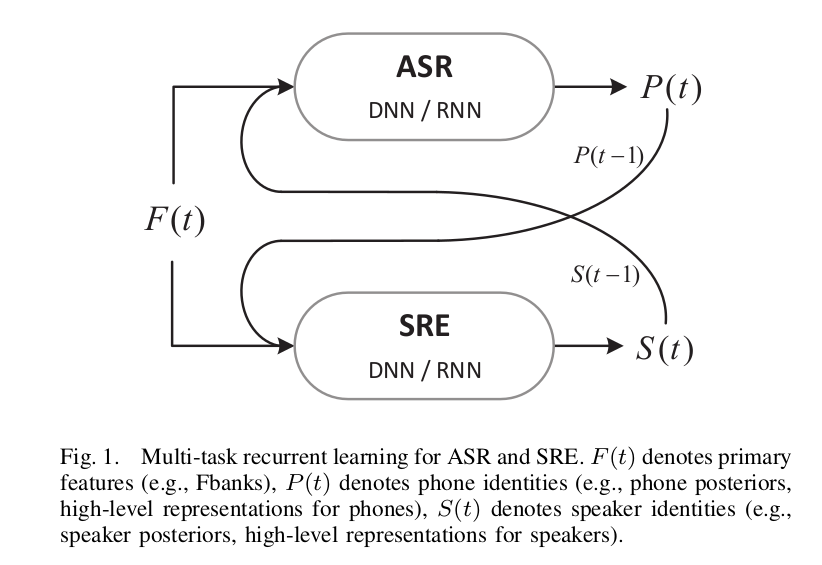
\includegraphics[width=0.75\linewidth]{images/multi-task-recurrent-learning.png}
		\label{fig:writing-thesis}
	\end{figure}
\end{frame}
\begin{frame}{Công trình tiêu biểu sử dụng Multi-domain features}
	\textbf{Phương pháp thực hiện}: Ý tưởng cơ bản của nó là sử dụng đầu ra của một tác vụ như một đầu vào vào của những tác vụ khác (khá tương tự với kiến trúc RNN thông thường). Kết quả đầu ra của một tác vụ ở bước thời gian trước đó $t-1$ được sử dụng để cung cấp cho một tác vụ ở thời điểm $t$ hiện tại.
	\begin{figure}[H]
		\centering
		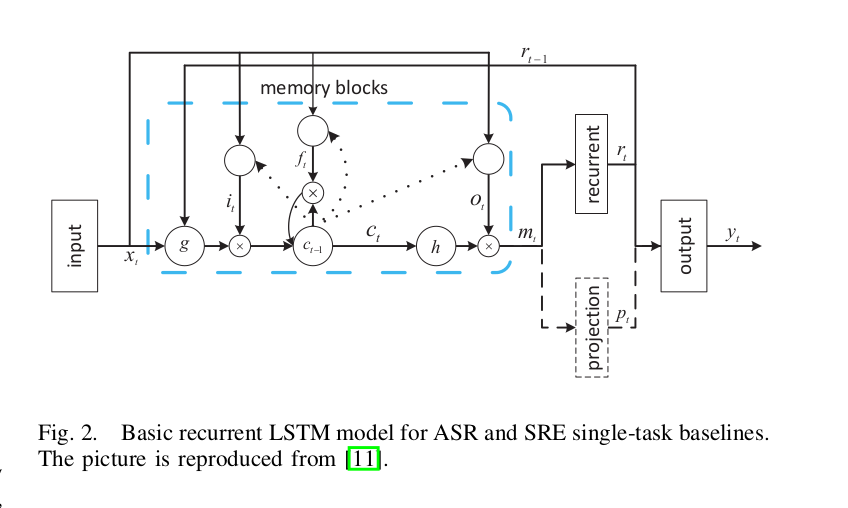
\includegraphics[width=0.75\linewidth]{images/basis-single-task-model.png}
		\label{fig:writing-thesis}
	\end{figure}
\end{frame}
\begin{frame}{Công trình tiêu biểu sử dụng Multi-domain features}
	\textbf{Các kết quả đạt được}
	\begin{columns}
		\begin{column}{0.5\textwidth}
			\begin{figure}[H]
				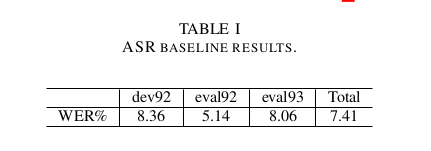
\includegraphics[width=0.8\linewidth]{images/multi-task-recurrent-model-asr-baseline-res.png}
			\end{figure}
			\begin{figure}[H]
				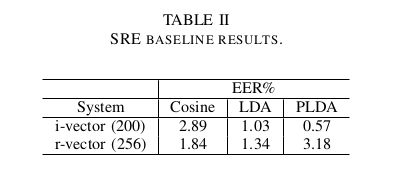
\includegraphics[width=0.8\linewidth]{images/multi-task-recurrent-model-sre-baseline-res.png}
			\end{figure}
		\end{column}
		\begin{column}{0.5\textwidth}
			\begin{figure}[H]
				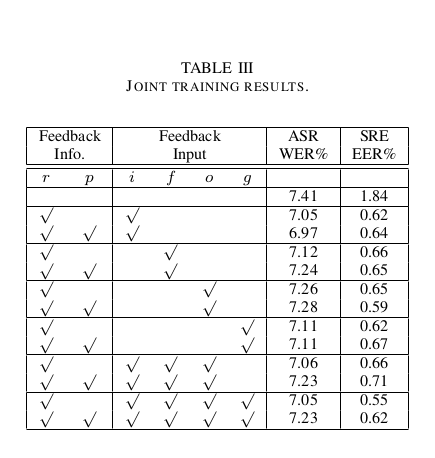
\includegraphics[width=0.75\linewidth]{images/multi-task-recurrent-model-joint-training-res.png}
			\end{figure}
		\end{column}
	\end{columns}
	\textbf{Nhận xét}
	\begin{itemize}
		\item Một kiến trúc mạng học lặp lại có thể huấn luyện cùng lúc nhiều tác vụ.
		\item Kết quả trên cơ sở dữ liệu cho thấy nhiều triễn vọng cho kiến trúc nói riêng, và những hướng hướng tiếp cận đa nhiệm nói chung.
	\end{itemize}
\end{frame}
\begin{frame}{Công trình tiêu biểu: SincNet}
	\textbf{Giới thiệu chung về bài báo:}
	\begin{itemize}
		\item Bài báo: Speaker Recognition from Raw waveform with SincNet
		\item Nhóm tác giả: Mirco Ravanelli, Yoshua Bengio*
		\begin{itemize}
			\item Mila, Université de Montréal
			\item CIFAR Fellow*
		\end{itemize}
		\item Được công bố trên arXiv.org vào năm 2018
	\end{itemize}
\end{frame}
\begin{frame}{Công trình tiêu biểu sử dụng SincNet}
	\textbf{Mô hình}
	\begin{figure}[H]
		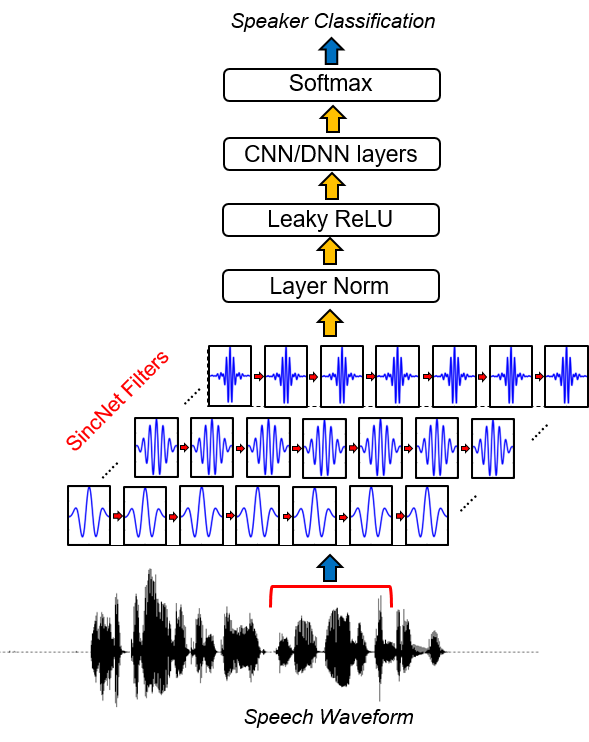
\includegraphics[width=0.4\linewidth]{images/SincNet.png}
		\caption{The SincNet Architecture}
		\label{fig:writing-thesis}
	\end{figure}
\end{frame}
\begin{frame}{Công trình tiêu biểu: SincNet}
	\textbf{Phương pháp thực hiện} Sincnet thực hiện các phép tích chập của nó với hàm $g$, hàm này phụ thuộc vào một tham số $\theta$. Công thức như sau:
	
	$$y[n] = x[n] * g[n, \theta]$$
	
	Trong xử lý tín hiệu số, $g$ được định nghĩa như một filter-bank gồm các bộ lọc (filter) băng thông hình chữ nhật. Trong miền tần số, độ lớn của một bộ lọc băng thông tổng quát có thể được tính như hiệu số giữa 2 bộ lọc thông tần số thấp
	
	Với $f_1$ $f_2$ lần lượt là tần số cắt thấp (low) và cao (high) đã được học, $rect(.)$ là hàm rectangular trong miền tần số.
	
	\begin{gather*}
		G[f, f_1, f_2] = rect\left(\frac{f}{2f_2}\right) -  rect\left(\frac{f}{2f_1}\right)\\ \xrightarrow{\text{Fourier Inverse}}g[n, f_1, f_2] = 2f_2sinc(2\pi f_2 n) - 2f_1sinc(2\pi f_1 n)
	\end{gather*}
\end{frame}
\begin{frame}{Công trình tiêu biểu: SincNet}
	\textbf{Các kết quả đạt được}\newline
	\begin{columns}
		\begin{column}{0.5\textwidth}
			Speaker Identification Task
			\begin{figure}[H]
				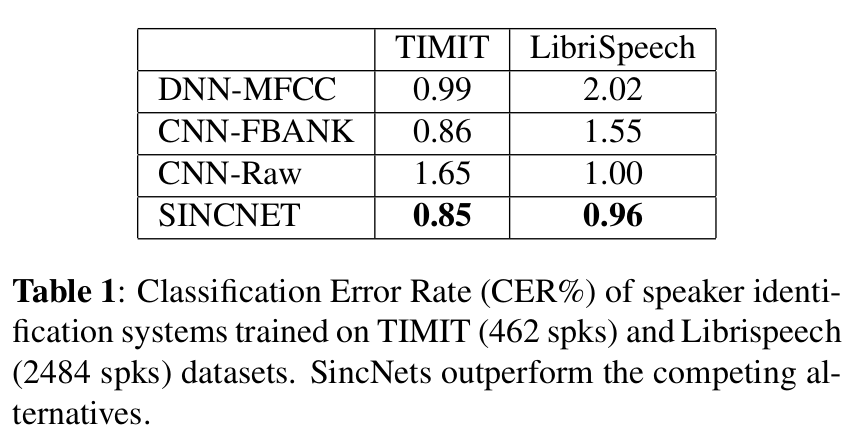
\includegraphics[width=1\linewidth]{images/performance_speaker_identification.png}
			\end{figure}
		\end{column}
		\begin{column}{0.5\textwidth}
			Speaker Verification Task
			\begin{figure}[H]
				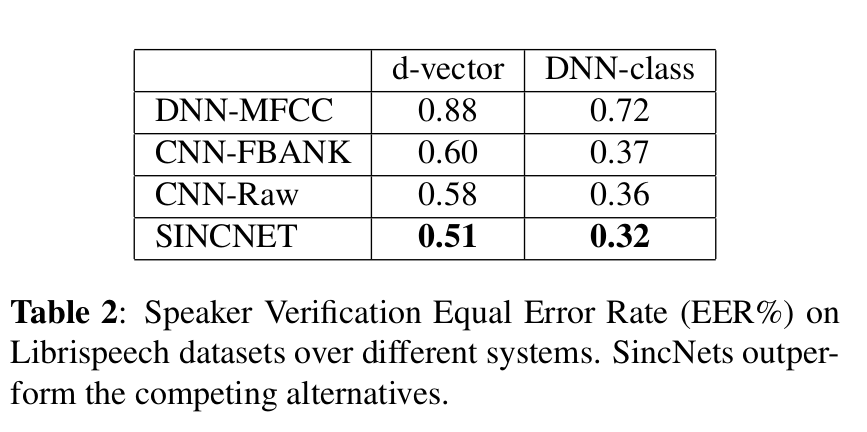
\includegraphics[width=1\linewidth]{images/performance_speaker_verification.png}
			\end{figure}
		\end{column}
	\end{columns}
	\textbf{Nhận xét}
	\begin{itemize}
		\item Cơ sở lý thuyết Toán học vững vàng
		\item Tính toán nhanh và gọn nhẹ
		\item Kết hợp với Deep Learning một cách hiệu quả: Sử dùng DNN-Class trong đánh giá, cho kết quả đầy khả quan, có độ lỗi EER thấp
	\end{itemize}
\end{frame}
\subsection{Thực nghiệm}
\begin{frame}{Thực nghiệm}
	\huge Phần thực hành demo với SincNet
\end{frame}
\subsection{Tài liệu tham khảo - References}
\begin{frame}
	\nocite{*}
	\bibliography{references}\newpage\cleardoublepage
	\bibliographystyle{plain}
\end{frame}

\end{document}